%%
%% Apendice.tex
%% Projeto Oficinas de Integração 3
%% Created by Leonardo Winter Pereira and Lucas Zimmermann Cordeiro on 10.03.2016
%% Copyright (C). All rights reserved
%%

%% Apêndice é um texto ou documento elaborado pelo autor do TC, ou seja,
%% se foi necessário você criar uma entrevista, um relatório, ou qualquer
%% documento com o escopo de complementar sua argumentação


\chapter{Nome do Apêndice}

    \section{Notas musicais em MIDI}
    
        O estudo da música em si está fora do escopo deste projeto. Entretanto, é imprescindível entender o que é uma oitava. Segue uma breve definição: \epigraph{Uma oitava é o intervalo entre uma nota musical e outra com a metade ou o dobro de sua frequência.}{~\cite{WikipediaOitava}}
        
        Dizer que uma nota está uma oitava acima significa dizer que a nota é a mesma, porém ela está em uma região mais aguda do instrumento.
    
        \definecolor{darkRed}{rgb}{0.607843137254902, 0.1764705882352941, 0.1215686274509804}
        \definecolor{lightRed}{rgb}{0.9568627450980392, 0.803921568627451, 0.7843137254901961}
        
        \begin{table}[H]
            \centering
            \begin{tabular}{| c | c | c | c | c | c | c | c | c | c | c | c | c |}
                \hline
                %\rowcolor{darkRed} \textcolor{white}{\textbf{Oitava}} & \textcolor{white}{\textbf{Número referente a nota}} \\
                \rowcolor{darkRed} \textcolor{white}{\textbf{Oitava}} & \textcolor{white}{\textbf{C}} & \textcolor{white}{\textbf{C\#}} & \textcolor{white}{\textbf{D}} & \textcolor{white}{\textbf{D\#}} & \textcolor{white}{\textbf{E}} & \textcolor{white}{\textbf{F}} & \textcolor{white}{\textbf{F\#}} & \textcolor{white}{\textbf{G}} & \textcolor{white}{\textbf{G\#}} & \textcolor{white}{\textbf{A}} & \textcolor{white}{\textbf{A\#}} & \textcolor{white}{\textbf{B}} \\
                \hline
                \rowcolor{lightRed} \textbf{-1} &  0   & 1   & 2   & 3   & 4   & 5   & 6   & 7   & 8   & 9   & 10 & 11 \\
                \hline
                \rowcolor{white}     \textbf{0} &  12  & 13  & 14  & 15  & 16  & 17  & 18  & 19  & 20  & 21  & 22 & 23 \\
                \hline
                \rowcolor{lightRed}  \textbf{1} &  24  & 25  & 26  & 27  & 28  & 29  & 30  & 31  & 32  & 33  & 34 & 35 \\
                \hline
                \rowcolor{white}     \textbf{2} &  36  & 37  & 38  & 39  & 40  & 41  & 42  & 43  & 44  & 45  & 46 & 47 \\
                \hline
                \rowcolor{lightRed}  \textbf{3} &  48  & 49  & 50  & 51  & 52  & 53  & 54  & 55  & 56  & 57  & 58 & 59 \\
                \hline
                \rowcolor{white}     \textbf{4} &  60  & 61  & 62  & 63  & 64  & 65  & 66  & 67  & 68  & 69  & 70 & 71 \\
                \hline
                \rowcolor{lightRed}  \textbf{5} &  72  & 73  & 74  & 75  & 76  & 77  & 78  & 79  & 80  & 81  & 82 & 83 \\
                \hline
                \rowcolor{white}     \textbf{6} &  84  & 85  & 86  & 87  & 88  & 89  & 90  & 91  & 92  & 93  & 94 & 95 \\
                \hline
                \rowcolor{lightRed}  \textbf{7} &  96  & 97  & 98  & 99  & 100 & 101 & 102 & 103 & 104 & 105 & 106 & 107 \\
                \hline
                \rowcolor{white}     \textbf{8} &  108 & 109 & 110 & 111 & 112 & 113 & 114 & 115 & 116 & 117 & 118 & 119 \\
                \hline
                \rowcolor{lightRed}  \textbf{9} &  120 & 121 & 122 & 123 & 124 & 125 & 126 & 127 &     &     &     &     \\
                \hline
            \end{tabular}
            \caption{Notas musicais em MIDI}
            \label{table:MIDI_notes}
        \end{table}

%% ---------------- 4 -------------------
%% O Gerenciamento da Integração do Projeto descreve os processos necessários para assegurar que os diversos elementos do projeto sejam adequadamente coordenados.
%% A integração envolve tomada de decisão e escolhas diretamente ligadas aos objetivos do projeto e aos processos das etapas de desenvolvimento e execução do plano do projeto, assim como ao processo de controle de alterações.
%% O gerenciamento da integração é composto pelos processos: desenvolvimento do plano do projeto, execução do plano do projeto e controle integrado de mudanças
%\chapter{Gerenciamento de Integração do Projeto}



    %% ---------------- 4.1 -------------------
%    \section{Termo de Abertura do Projeto}

%    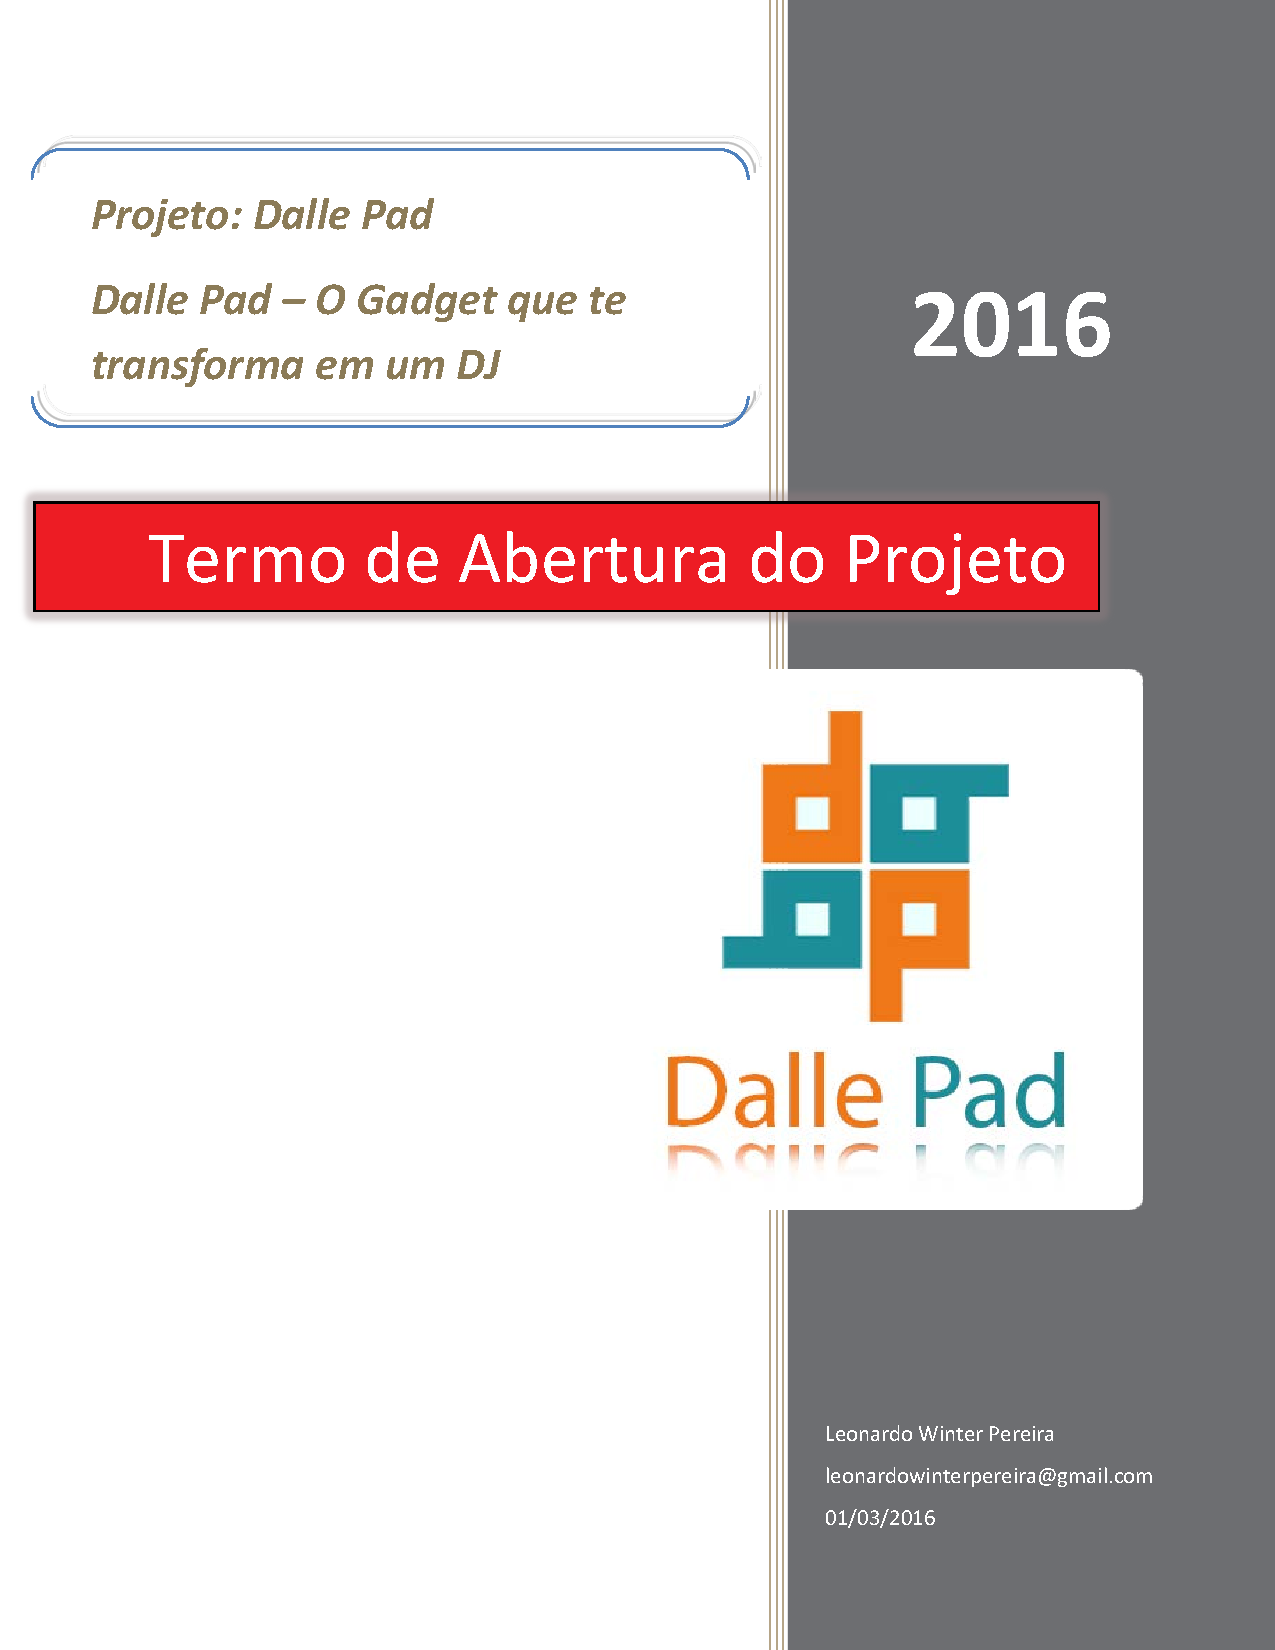
\includepdf[pages={-}]{Documentos/Termo_de_Abertura_de_Projeto.pdf}

    %% ---------------- 4.2 -------------------
%    \section{Declaração do Escopo Preliminar do Projeto}



    %% ---------------- 4.3 -------------------
%    \section{Plano de Gerenciamento do Projeto}

%    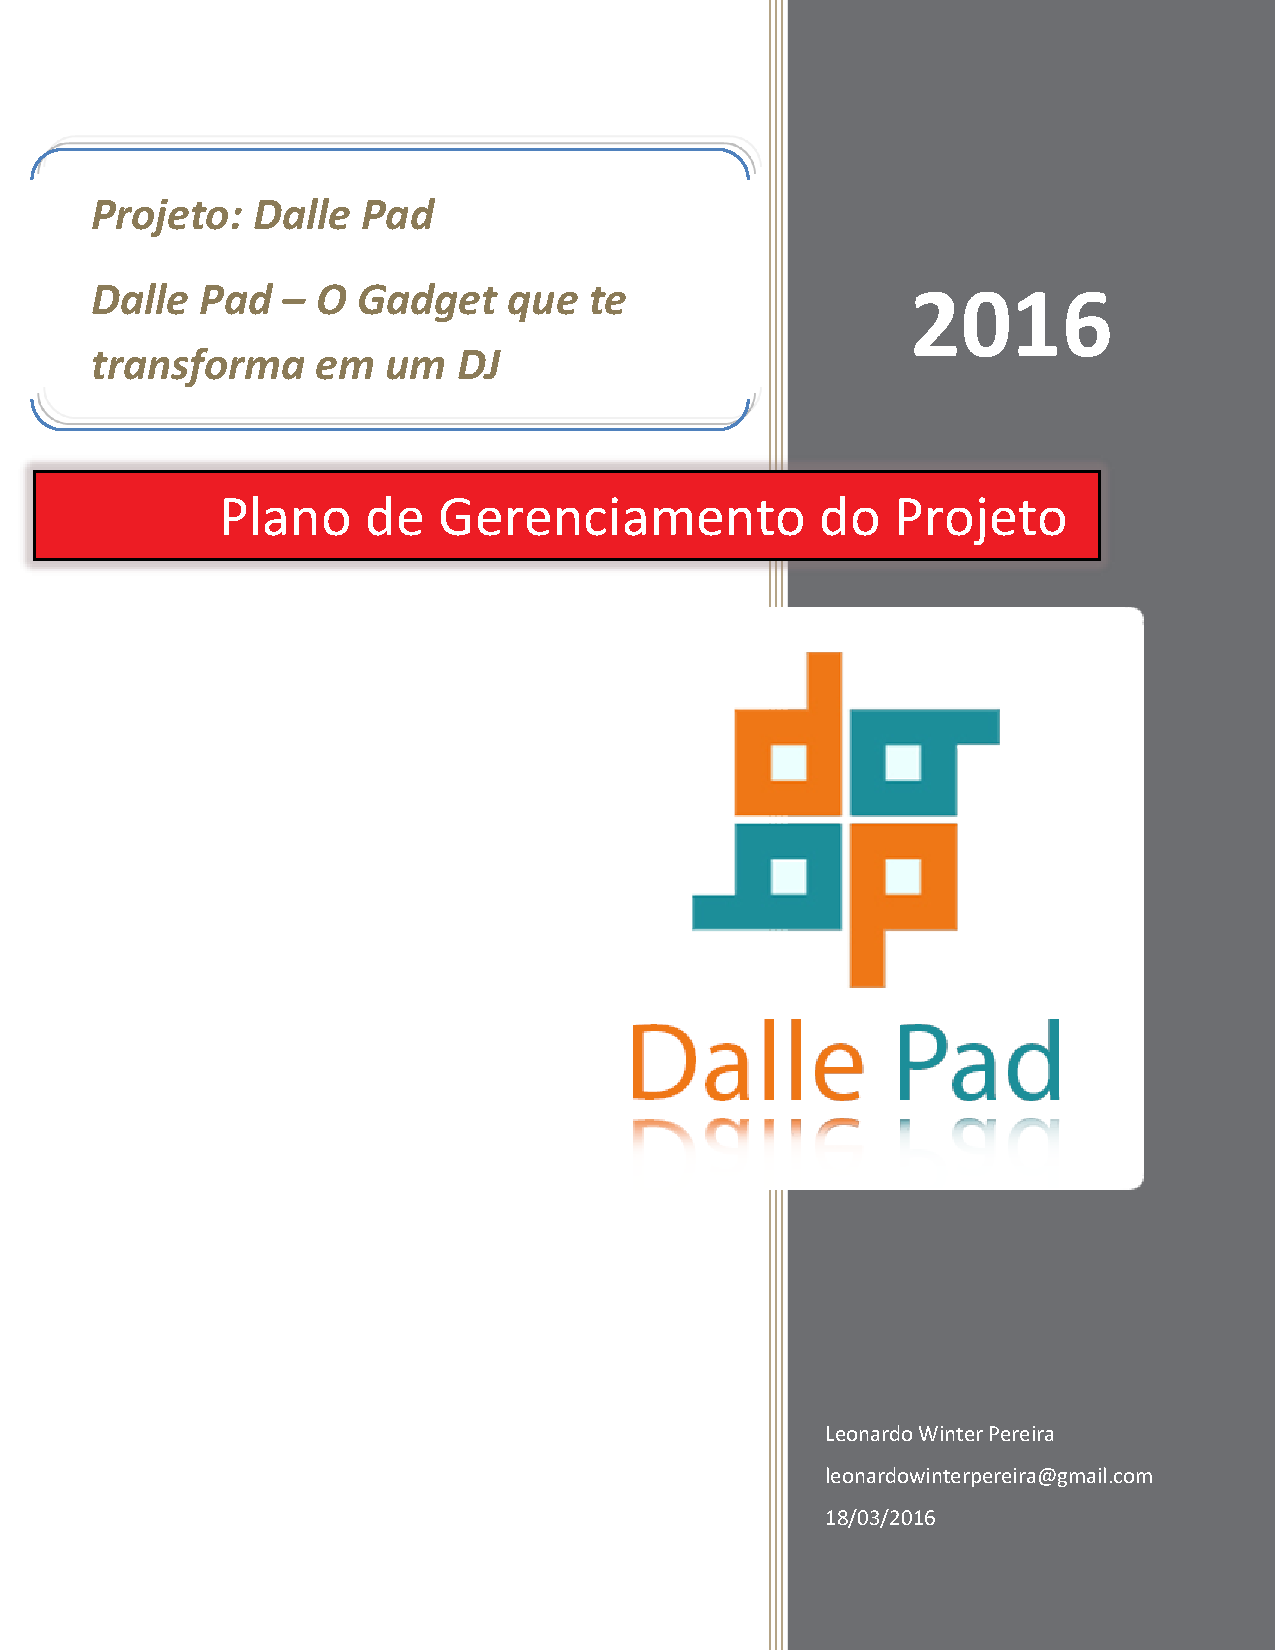
\includepdf[pages={-}]{Documentos/Plano_de_Projeto.pdf}

%% ---------------- 5 -------------------
%% O Gerenciamento do Escopo do Projeto descreve os processos necessários para assegurar que o projeto contemple todo o trabalho requerido, e nada mais que o trabalho requerido, para completar o projeto com sucesso.
%% A preocupação fundamental é definir e controlar o que está ou não, incluído no projeto.
%% Ele é composto pelos processos: iniciação, planejamento do escopo, detalhamento do escopo, verificação do escopo e controle de mudanças do escopo.
%\chapter{Gerenciamento de Escopo do Projeto}



    %% ---------------- 5.1 -------------------
%    \section{Planejamento do Escopo}



    %% ---------------- 5.2 -------------------
%    \section{Definição do Escopo}



    %% ---------------- 5.3 -------------------
%    \section{Estrutura Analítica do Projeto}



%% ---------------- 6 -------------------
%% O Gerenciamento do Tempo do Projeto descreve os processos necessários para assegurar que o projeto termine dentro do prazo previsto.
%% Ele é composto pelos processos: definição das atividades, sequenciamento das atividades, estimativa da duração das atividades, desenvolvimento do cronograma e controle do cronograma.
%\chapter{Gerenciamento do Tempo do Projeto}



    %% ---------------- 6.1 -------------------
%    \section{Definição da Atividade}



    %% ---------------- 6.2 -------------------
%    \section{Sequenciamento de Atividades}



    %% ---------------- 6.3 -------------------
%    \section{Estimativa de recursos de atividade}



    %% ---------------- 6.4 -------------------
%    \section{Estimativa de duração de atividade}



    %% ---------------- 6.5 -------------------
%    \section{Desenvolvimento do Cronograma}



%% ---------------- 7 -------------------
%% O Gerenciamento do Custo do Projeto descreve os processos necessários para assegurar que o projeto termine dentro do orçamento aprovado.
%% Ele é composto pelos processos: planejamento dos recursos, estimativa dos custos, orçamento dos custos e controle dos custos.
%% No projeto, várias atividades afetam os custos do projeto e desta forma, o planejamento e controle dos custos são fundamentais.
%\chapter{Gerenciamento do Custo do Projeto}



    %% ---------------- 7.1 -------------------
%    \section{Estimativa de custos}



    %% ---------------- 7.2 -------------------
%    \section{Orçamentação}



%% ---------------- 8 -------------------
%% O Gerenciamento da Qualidade do Projeto descreve os processos necessários para assegurar que as necessidades que originaram o desenvolvimento do projeto serão satisfeitas.
%% O projeto tem qualidade quando é concluído de acordo com os requisitos, especificações (o projeto deve produzir o que foi definido) e adequação ao uso (deve satisfazer às reais necessidades dos clientes).
%% O gerenciamento da qualidade é composto pelos processos: planejamento da qualidade, garantia da qualidade e controle da qualidade.
%\chapter{Gerenciamento da Qualidade do Projeto}



    %% ---------------- 8.1 -------------------
%    \section{Planejamento da qualidade}



%% ---------------- 9 -------------------
%% O Gerenciamento dos Recursos Humanos do Projeto descreve os processos necessários para proporcionar a melhor utilização das pessoas envolvidas no projeto. Embora seja uma área de conhecimento, na maioria das vezes, complexa e subjetiva exige constante pesquisa, sensibilidade e muita vivência do dia-a-dia para saber lidar com o ser humano.
%% É composta pelos processos: planejamento organizacional, montagem da equipe e desenvolvimento da equipe.
%\chapter{Gerenciamento de Recursos Humanos do Projeto}



    %% ---------------- 9.1 -------------------
%    \section{Planejamento de recursos humanos}



%% ---------------- 10 -------------------
%% O Gerenciamento das Comunicações do Projeto descreve os processos necessários para assegurar a geração, captura, distribuição, armazenamento e pronta apresentação das informações do projeto para que sejam feitas de forma adequada e no tempo certo.
%% A gestão da comunicação é frequentemente ignorada pelos gerentes de projeto, no entanto nos projetos concluídos com sucesso o gerente gasta 90% do seu tempo envolvido com algum tipo de comunicação (formal, informal, verbal, escrita).
%% Este gerenciamento é composto pelos processos: planejamento das comunicações, distribuição das informações, relato de desempenho e encerramento administrativo
%\chapter{Gerenciamento de Comunicação do Projeto}



    %% ---------------- 10.1 -------------------
%    \section{Planejamento das comunicações}



%% ---------------- 11 -------------------
%% O Gerenciamento dos Riscos do Projeto descreve os processos que dizem respeito à identificação, análise e resposta aos riscos do projeto.
%% A prática deste gerenciamento não é ainda muito comum na maioria das organizações e alguns autores citam que gerenciar projetos é gerenciar riscos.
%% O gerenciamento de riscos é muito importante para o sucesso do projeto e é composto pelos seguintes processos: Planejamento da Gerência de Risco, identificação dos riscos, análise qualitativa de riscos, análise quantitativa de riscos, desenvolvimento das respostas aos riscos e controle e monitoração de riscos.
%\chapter{Gerenciamento do Risco do Projeto}



    %% ---------------- 11.1 -------------------
%    \section{Planejamento do gerenciamento de riscos}



    %% ---------------- 11.2 -------------------
%    \section{Identificação de riscos}



    %% ---------------- 11.3 -------------------
%    \section{Análise Qualitativa de riscos}



    %% ---------------- 11.4 -------------------
%    \section{Planejamento de respostas a riscos}



%% ---------------- 12 -------------------
%% O Gerenciamento das Aquisições do Projeto descreve os processos necessários para a aquisição de mercadorias e serviços fora da organização que desenvolve o projeto.
%% Este gerenciamento é discutido do ponto de vista do comprador na relação comprador-fornecedor.
%% Ele é composto pelos processos: planejamento das aquisições, preparação das aquisições, obtenção de propostas, seleção de fornecedores, administração dos contratos e encerramento do contrato.
%\chapter{Gerenciamento das Aquisições do Projeto}



    %% ---------------- 12.1 -------------------
%    \section{Planejar compras e aquisições}



    %% ---------------- 12.2 -------------------
%    \section{Planejar contratações}



%% Atas de Reunião são importantes pois definem exatamente o que foi / será discutido em cada reunião da Equipe Dalle Pad!
%\chapter{Atas de Reunião}


